
\section{The basic model}
\label{basicModel}

\subsection{Pitman-Yor Process}

The Pitman-Yor process is a generalization of the Dirichlet process and is a distribution over distributions with three parameters.  If $\G_1 \sim \PY(d,c,\G_0)$ we say $\G_1$ is distributed according to a Pitman-Yor process with discount parameter $d$, concentration parameter $c$, and base measure $\G_0$. The Pitman-Yor process reduces to the Dirichlet process when $d = 0$ \cite{Pitman}. 

The Pitman-Yor process can also be reformulated by analytically marginalizing out the random distribution $\G_1$.  To draw a sample $\{ \theta_j \}_{j = 1}^N$ in this representation we use a two step process.  The first step is to obtain a partition of the first $N$ integers from the two parameter Ewen's sampling distribution ($\ES_N(d,c)$).  The second step is to endow each of the $K$ parts of the partition with a parameter $\psi_k$ drawn independently from $\G_0$.  We define $\theta_j = \psi_k$ for all integers $j$ in the $k$'th section of the partion \cite{mcqueen??}.

The two parameter Ewen's sampling distribution is most easily understood through the process by which a sample is generated.  The process is known as the Chinese restaurant process (CRP) because of the metaphor that integers correspond to customers being seating in a restaurant with infinitely many tables.  Since the details of this process are critical for extensions made later we need to describe the CRP in detail. The process is initialized by seating the first customer at an empty table.  Customers $2 \dots N$ are seated sequentially by seating the $j$'th customer at a table drawn from the following distribution:

\begin{eqnarray*}
p(\textrm{table}_i, i<= t_{j-1} |\textrm{ previous customers}) &=& \frac{n_i - d}{j-1+ c}\\
p(\textrm{table}_{t_{j-1} +1} | \textrm{ previous customers}) &=& \frac{t_{j-1}d +c}{j-1+c}
\end{eqnarray*}

where $n_i$ is the number of customers already sitting at table $i$ and $t_{j-1}$ is the number of tables occupied by the first $j-1$ customers.  The final state of the restaurant defines a partition over the first $N$ integers which follows the $\ES_N(d,c)$ distribution.  Step two of the algorithm above is achieved by endowing each table with a parameter $\psi_k$ drawn independently from $\G_0$.

%TODO need a figure here to show restaurants arranged.  rest 1 will be the upper restaurant, rest 2 will be the lower restaurant.
These random distributions can be arranged in a hierarchy, such as the case that $\G_2 \sim \PY(d_2, c_2, \G_1)$ and $\G_1 \sim \PY(d_1, c_1, \G_0)$.  The hierarchical process can also be reformulated by analytically marginalizing out both $\G_2$ and $\G_1$.  Samples are obtained by iterating the algorithm for the single Pitman-Yor process.  To draw a sample $\{ \theta_j \}_{j = 1}^N$ we again need to obtain a partition of the first $N$ integers from $\ES_N(d,c)$.  This can be achieved through the CRP.  We will call this restaurant the child restaurant and denote the number of tables as $K_2$.  Each of the $K_2$ tables must be endowed with a parameter $ \psi_{2k}$ drawn independently from $\G_1$.  Since $\G_1$ has been marginalized out we can obtain $\{ \psi_{2k} \}_ {k = 1}^{K_2}$ by again using the algorithm for the single Pitman-Yor process.  A partition from the $\ES_{K_2}(d,c)$ is generated via the CRP.  We will call this restaurant the parent restaurant and the number of tables $K_1$.   Each of the $K_1$ tables must be endowed with a parameter $\psi_{1k}, k = 1 \ldots K_1$,  independently drawn from $\G_0$.  The sample consists of $\theta_j =\psi_{2k}$ for all customers $j$ sitting at table $k$ in the the child restaurant.

\begin{figure}[h!tbp] 
	\begin{center}
		\scalebox{.25}{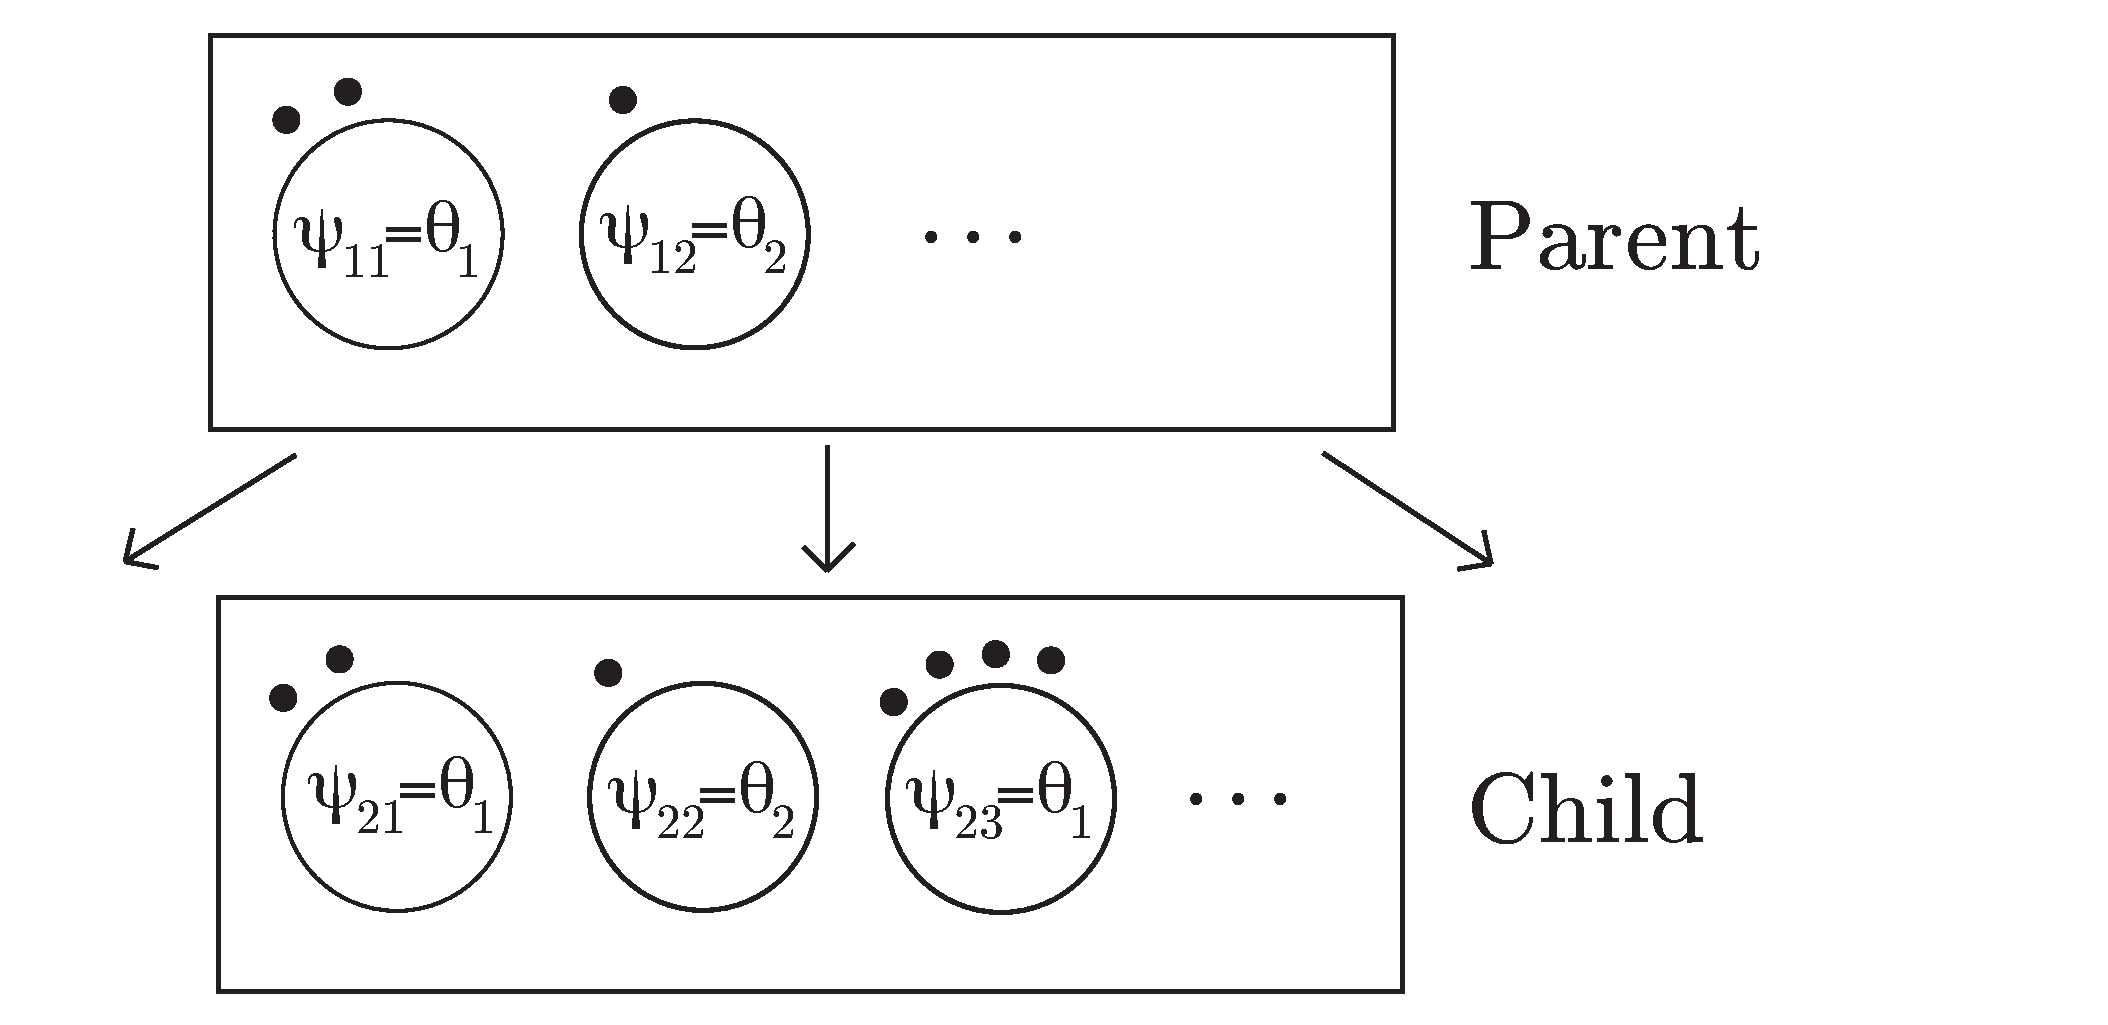
\includegraphics{figure1.pdf}} % [clip=true, viewport= 1in 1in 9in 9in]
		\caption{Final state of an example CRF process.}
	\end{center} 
	\label{figHPY}
\end{figure} 

The process is most easily understood by looking at Figure~\ref{figHPY} in which the CRP process for the child restaurant resulted in three tables ($K_2 = 3$).  Therefore, three parameters must be drawn from $\G_1$.  Since $\G_1$ is marginalized we again revert to the process for a single Pitman-Yor process. The CRP for the parent restaurant resulted in two tables ($K_1 = 2$).  $\psi_{11}$ and $\psi_{12}$ are drawn independently from the base distribution $\G_0$.  $\{ \psi_2k \}_{k = 1}^{K_1}$ is then equal to $\{ \theta_1, \theta_1, \theta_2 \}$ which are then the parameters endowed to tables in the child restaurant.  From the figure we find that  $\{ \theta_j \}_{j = 1}^7 = \{ \theta_1, \theta_1, \theta_2, \theta_1, \theta_1, \theta_1, \theta_1 \}$.

The iterative application of the CRP representation is known as the Chinese restaurant franchise (CRF) \cite{teh hdp paper}.  As alluded to in Figure~\ref{figHPY}, the number of child restaurants is not restricted to one.  Furthermore, the iterative nature of the process makes extensions to deeper hierarchies natural.  For more extensive coverage of these representations we refer the reader to \cite{teh hpp} and \cite{teh hpy for langmodel}.

\subsection{Sequence Memoizer}

The sequence memoizer (SM) \cite{wood}, is a hierarchical Pitman-Yor model of unbounded depth for discrete sequence data.  Each node in the graphical model represents the distribution over the set of types ($\Sigma$) conditioned by a unique context.  The context consists of the entire sequence of types preceding the observation.  We can write the model as:

\begin{eqnarray*}
	\G_{[]} | \mathcal{U}_{\Sigma}, d_0 &\sim& \PY(d_0, 0, \mathcal{U}_{\Sigma }) \\
	\G_{\bf{u}} | \G_{\sigma(\bf{u})}, d_{|\bf{u}|} &\sim& \PY(d_{|\bf{u}|}, 0, \G_{\sigma(\bf{u})}) \hspace{1cm} \forall \bf{u} \in \Sigma^+
\end{eqnarray*}

where $\mathcal{U}_{\Sigma }$ is a uniform distribution over the set of types, $\bf{u}$ is a particular context, $\Sigma^+$ is the set of all such contexts, and $\sigma(\bf{u})$ is the context $\bf{u}$ modified by removing the most distant type.  We assume $| \Sigma | < \infty$.

In \cite{pitman} they show that  if $\G_2 \sim \PY(d_2, 0, \G_1)$ and  $\G_1 \sim \PY(d_1, 0, \G_0)$ then marginally, $\G_2 \sim \PY(d_2 d_2, 0, \G_0)$.  \cite{wood} applied this result to show that the graphical model for the SM to be identified in linear time and initiated in linear space.

Inference in the SM model is performed in the Chinese restaurant franchise respresentation. Inference takes worst case $\mathcal{O}(n^2)$ time and requires $\mathcal{O}(n)$ space. Quadratic time stems from the fact that seating a customer in the appropriate restaurant may require seating a customer in all of the restaurants above it.  The length of this path is bounded by the length of the sequence. Each restaurant requires constant space because a restaurant need only maintain a constant number of summary statistics, the total number of customers and the total number of tables present of each type.\footnote{For symbol sets of finite cardinality.} Note this representation requires reinstantiation of the full restaurant state for some steps of inference which can be done by exploiting exchangeability.
